\documentclass[border=10pt]{standalone}

\usepackage{tikz}
\usepackage{tikzsymbols}
\usetikzlibrary{calc,patterns,shapes.geometric}

\def\centerarc[#1](#2)(#3:#4:#5){\draw[#1] ($(#2)+({#5*cos(#3)},{#5*sin(#3)})$) arc (#3:#4:#5);}

\begin{document}
	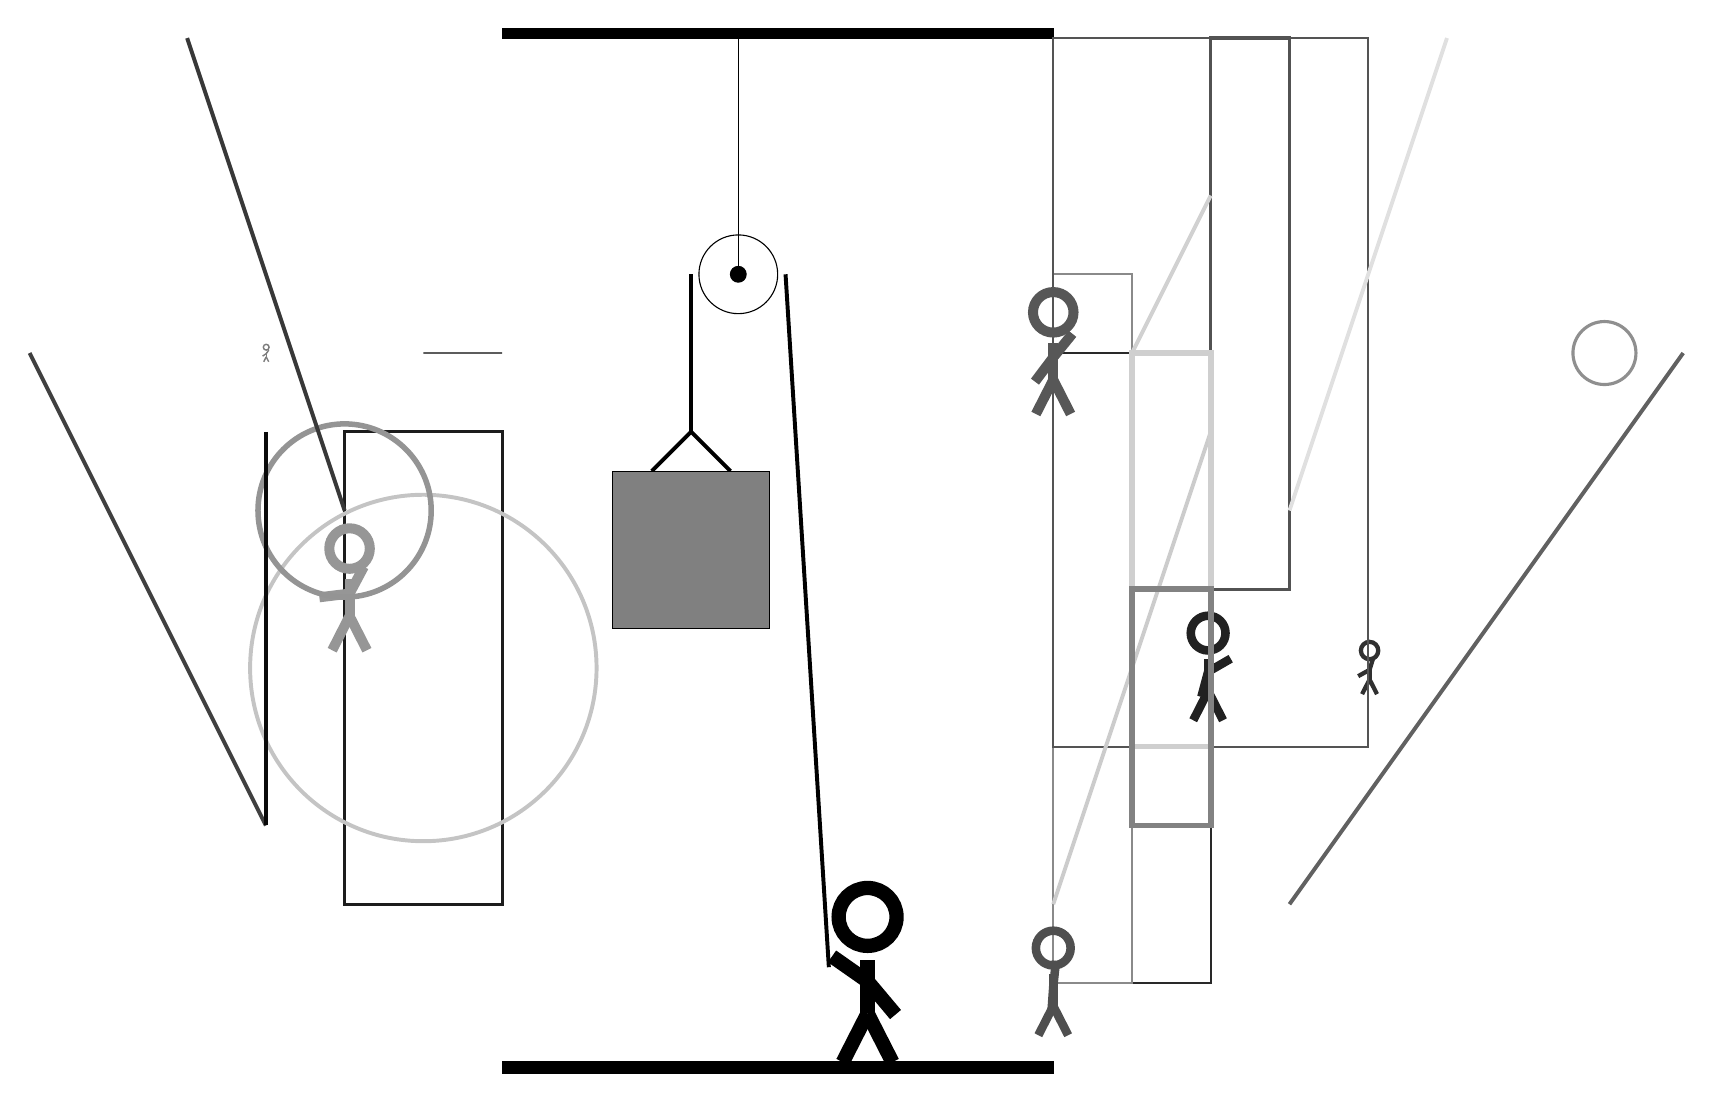
\begin{tikzpicture}
		%%%%% START %%%%%
		
		\draw[fill=black] (-2, 10) rectangle (5, 10.125);
		
		\draw (1, 7) circle (0.5);
		\draw[fill=black] (1, 7) circle (0.1);
		\draw (1, 10) -- (1, 7);
		
		\draw[line width=0.5mm] (-0.1, 4.5) -- (0.4, 5.0) -- (0.9, 4.5);
		\draw[fill=black!50] (-0.6, 4.5) rectangle (1.4, 2.5);
		
		\draw[line width=0.5mm] (0.4, 7) -- (0.4, 5.0);
		\centerarc[line width=0.5mm](1, 7)(0:180:0.6);
		\draw[line width=0.5mm](1.6, 7) -- (2.15, -1.8);
		
		\node at (2.6, -1.9) {\Strichmaxerl[10][-35][-50]};
		
		\draw[line width=0.4mm, color=black!68] (7, 10) rectangle (8, 3);
		
		\draw[line width=0.4mm, color=black!89] (-2, 5) rectangle (-4, -1);
		\draw[line width=0.3mm, color=black!84] (5, -2) rectangle (7, 6);
		\node[line width=0.6mm, color=black!87] at (7, 2) {\Strichmaxerl[6][75][30]};
		\draw[line width=0.5mm, color=black!75](-5, 0) -- (-8, 6);
		
		\draw[line width=0.5mm, color=black!62](8, -1) -- (13, 6);
		\node[line width=0.6mm, color=black!41] at (-4, 3) {\Strichmaxerl[7][7][62]};
		\draw[line width=0.3mm, color=black!46] (5, -2) rectangle (6, 7);
		\node[line width=0.5mm, color=black!81] at (9, 2) {\Strichmaxerl[3][29][73]};
		\node[line width=0.3mm, color=black!51] at (-5, 6) {\Strichmaxerl[1][34][54]};
		\draw[line width=0.3mm, color=black!67] (5, 1) rectangle (9, 10);
		\node[line width=0.4mm, color=black!66] at (5, 6) {\Strichmaxerl[7][53][51]};
		\node[line width=0.2mm, color=black!69] at (5, -2) {\Strichmaxerl[6][86][84]};
		
		\draw[line width=0.5mm, color=black!20](7, 5) -- (5, -1);
		\draw[line width=0.2mm, color=black!64] (-2, 6) rectangle (-3, 6);
		\draw [line width=0.5mm, color=black!23](-3, 2) circle (2.2);
		
		\draw[line width=0.5mm, color=black!18](6, 6) -- (7, 8);
		\draw [line width=0.7mm, color=black!42](-4, 4) circle (1.1);
		\draw[line width=0.7mm, color=black!19] (7, 6) rectangle (6, 1);
		\draw[line width=0.5mm, color=black!12](10, 10) -- (8, 4);
		\draw [line width=0.4mm, color=black!44](12, 6) circle (0.4);
		
		\draw[line width=0.5mm, color=black!78](-4, 4) -- (-6, 10);
		\draw[line width=0.7mm, color=black!49] (6, 0) rectangle (7, 3);
		\draw[line width=0.5mm, color=black!96](-5, 5) -- (-5, 0);
		
		\draw[fill=black] (-2, -3) rectangle (5, -3.15);
		
		%%%%% END %%%%%
	\end{tikzpicture}
\end{document}